\documentclass[a4paper,12pt]{ctexart}
\usepackage{xeCJK}
\usepackage[backend = biber, style = gb7714-2015, url=false,gbtitlelink=true]{biblatex}
\usepackage{booktabs}
\usepackage{enumerate}
\usepackage{indentfirst}
\usepackage{graphicx}
\usepackage{longtable}
\usepackage[normalem]{ulem}
\usepackage{amsmath}
\usepackage{amsfonts}
\usepackage{amssymb}
\usepackage{float}
\usepackage{capt-of}
\usepackage{minted}
\usepackage[hidelinks]{hyperref}
\usepackage[table,xcdraw]{xcolor}
\author{董晨阳 \thanks{学号1800015446} 许天朗 \thanks{学号1800015428} 李昭伦 \thanks{学号1800015469}}
\date{\today}
\title{风管模型基金运行报告}
\begin{document}
\maketitle
\tableofcontents
\section{风险偏好和目标设定}
作为2021 年年底成立的新基金,本基金被动追踪一篮子股票的价值,持仓份额如表\ref{holdings} 所示。
\begin{table}[ht]
	\begin{tabular}{rrrrrrrrr}
		比亚迪    & 牧原股份    & 东方财富    & 温氏股份   & 宁德时代   \\
		0.0516 & -0.0129 & -0.0957 & 0.2051 & 0.0193 \\
		招商银行   & 中国平安    & 中国建筑    & 中国中免            \\
		0.0521 & 0.3665  & 0.3774  & 0.0366          \\
	\end{tabular}
	\caption{持仓份额}
	\label{holdings}
\end{table}

遵循一般私募基金运行惯例,本基金预警线设置为份额净值 0.8 元,止损线设置为份额净值 0.7 元。
触及预警线时,私募行业一般要求管理人及时减仓,直到净值重归预警线之上才能加仓。
触及止损线时,一般要求管理人无条件清仓,并将剩余的投资款返还客户。
双线作为一把“双刃剑”,一方面明确了安全边际,促使管理人谨慎投资并配置风控预案。另一方面,双线也加大了管理人在极端行情下的操作难度,大规模私募基金的减仓清盘行为甚至会加剧市场的波动。

本基金的业绩基准为沪深300 ETF。因而本基金的目标为在 300ETF 之上取得相对收益的同时,在四个月运行期间避免触及预警和清盘线。综上,本基金的风险偏好为每月最多亏损\(1-0.8^{1/4}\approx 0.05\),即每月净值下跌至多5\%。

本基金假定了股票交易成本为 0,期权价格采用二叉树公平定价。
\section{策略理由和面临的风险}
本基金持仓组合中的行业涉及金融、传统消费、新能源等行业,易受到整体经济运行环境的影响,当整体经济下行时,持仓组合中容易出现较大幅度的向下波动,因此我们选择通过购入反映整体股市波动的沪深300ETF进行对冲。我们采取 protective put 策略,即在持有股票的同时,每月月初在市场上购入适当的月末到期的、执行价格为95\% 的沪深300ETF 看跌期权。购入看跌期权。

每月具体1 单位基金的对冲期权数由两者的 \(\beta\) 计算得到。
计算结果如表 \ref{beta} 所示:
\begin{table}[htbp]
	\centering
	\begin{tabular}{ll}
		月份 & 1单位基金对冲期权数 \\\hline
		1月 & 0.4895       \\
		2月 & 0.5367       \\
		3月 & 0.5895       \\
		4月 & 0.8223       \\
	\end{tabular}
	\caption{\(\beta\) 变化}
	\label{beta}
\end{table}
我们的对冲策略面临的具体风险如下:
\begin{enumerate}
	\item 指数期权对冲效果不理想。
	      由于我国没有具体某只股票的期权,因此我们只能选择用指数期权对冲。存在指数与本基金基金相关性不强的风险,可能出现基金中标的资产下跌,指数上涨的情况,则会导致对冲效果不理想。
	\item 单位基金对冲数不足。
	      我们以月初计算得到的 \(\beta\) 值作为1单位基金的对冲期权数,实际上可能在月末行权时,我们计算得到的期权不能覆盖我们的损失,存在着对冲期权数不足的风险。
	\item 期权价格过高造成了较大的对冲成本。
	      我们每月初都会购入新的对冲期权,我们存在过度对冲的风险,由于期权的购买费用,给本基金的成本端造成了较大压力。
\end{enumerate}

\section{当前策略成果}
\begin{figure}[h]
    \centering
    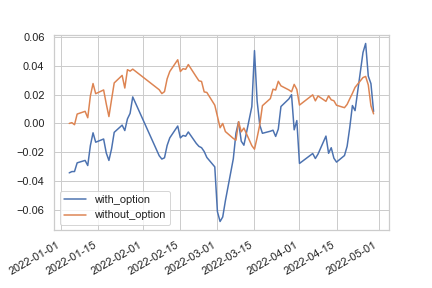
\includegraphics[width=0.8\linewidth]{./lib/result/result1.png}
    \caption{本基金相对于沪深300的超额收益}
    \label{fig:300etf}
\end{figure}
由图 \ref{fig:300etf}所示,两条曲线代表本基金在是否购买期权的两种状况下相对于沪深300ETF的超额收益。在购买期权这一策略下,每月月初将为购买期权付出一定的成本,因此两条曲线的差距在月初会一定程度上加大。
	根据这四个月的走势,当市场在小范围波动,未达到触发行权的条件时,购买期权的策略比不购买会获得更低的收益率。但在3月15日附近与4月底的两次大跌行情中,在看跌期权的保护下,本基金的收益率较大地超越了无期权保护的策略。
 
\begin{figure}[h]
    \centering
    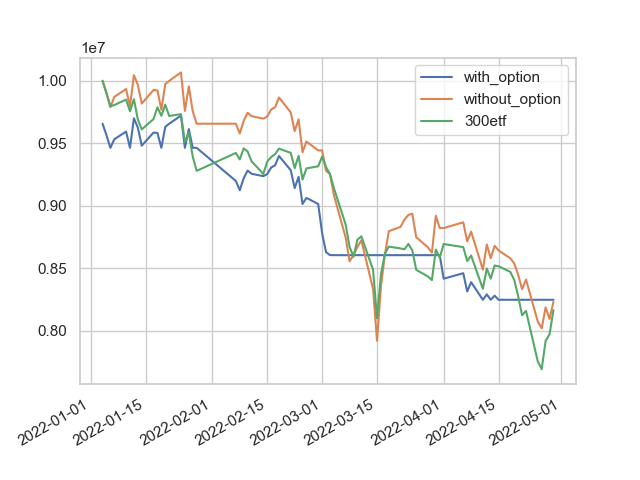
\includegraphics[width=0.8\linewidth]{./lib/result/result.png}
    \caption{市值波动}
    \label{fig:300}
\end{figure}
	
图 \ref{fig:300} 展示了三种策略下持有的市值在2022年1-4月期间的波动状况。策略包括持有本基金并购买看跌期权、只持有本基金、只持有沪深300ETF这三种。结果是,在2022年5月1 日,三种策略的市值相近,均相对于1月1日下跌了17\%左右。但是在有期权保护的策略下,市值的波动程度显著变小,在3月15日和4月底的两次大跌中都成功地平缓了曲线。Protective Put 策略成功起到了减小波动、稳定市值的作用。
 

\appendix
\section{代码说明}

src 目录下, config.py 与 markowitz.py 为上次作业确定组合头寸的代码。
pricing.py 中为建立二叉树从而对欧式/亚式/回望期权(包括 call \& put )定价的代码,使用时采用 partial 动态绑定。protective\_put.py 为本次作业的回测代码。

建议运行方式为
\begin{minted}{shell}
pip install poetry

poetry install 

poetry run python src/protective_put.py
\end{minted}

\end{document}
